\section{Using income and consumption to assess who is poor}\label{sec:composition}

%idea would be to move first bit of 4 and 5 into 3.

%Section \ref{sec:trends} showed that conclusions about the rate of growth in household resources in the UK, and the evolution of inequality and poverty, are sensitive to the way that resources are measured, but without exploiting that our data tells us about income and consumption for the same households. 

This section examines how income and consumption can give us different impressions of living standards for a given household.  We focus on the bottom of the distribution, and ask to what extent ``having a low income'' and ``having a low consumption'' identify different households (and, as background, Section \ref{subsec:ranks} shows the estimated rank correlations between the four measures of resources). This is clearly of prime importance for those interested in designing policies targeted at those with a low living standard. We do this for measures that do and do not include the imputed income or consumption from housing, with Section \ref{sec:housing} exploring how including the imputed income or consumption from housing affects which households are identified as being poor. We end by showing some suggestive evidence that ``having a low consumption'' is better correlated with other measures of living standards than ``having a low income''; this can be seen as complementary evidence to that in Brewer et al. (2016), which argued that the mismatch between income and spending at the bottom of the distribution seems likely to be caused by under-reporting of income than over-reporting of spending, or natural consumption smoothing in response to a volatile income flow. 

%showing that there are a sizeable number of individuals that are classified as ``poor'' when assessed using household income, but not when assessed using consumption measures (and vice versa)

\subsection{The mismatch between the ``income poor'' and the ``consumption poor''}\label{subsec:mismatch}

Figure \ref{fig:overlap} shows trends in the proportion of the population who are in both the bottom decile group of the distribution of income and the distribution of consumption (and calculated separately for measures that do and do not include imputed resources from housing); we refer to being in the bottom decile group of the distribution of income as being ``income poor'', and being in the bottom decile group of the distribution of consumption as being ``consumption poor''. A perfect rank correlation between income and consumption would mean that this fraction would be 10 percent.However, the average proportion of the population in the bottom decile groups of both of the distributions that do not include imputed income from housing was 2.32\% between 1979 and 2009.\footnote{The degree of overlap is even lower if we consider all four measures simultaneously: averaged over each year in our data, only 1.69\% of the population was in the bottom decile group of all four resource distributions.} This fraction is higher, at 3.96\%, and on an increasing trend, for the measures of resources that do include imputed resources from housing. This reflects that the two IHC measures are (weakly) positively correlated by construction (because we add to each the same impited value of income or consumption from housing), and the fact that the fraction deemed poor on both is rising over time when using a resource measure that includes the imputed resources from housing reflects that the amount of imputed income from housing is growing in importance at the bottom of the resource distribution.

\begin{figure}
\caption{In Bottom Decile of Income and Consumption Distributions}
\centering
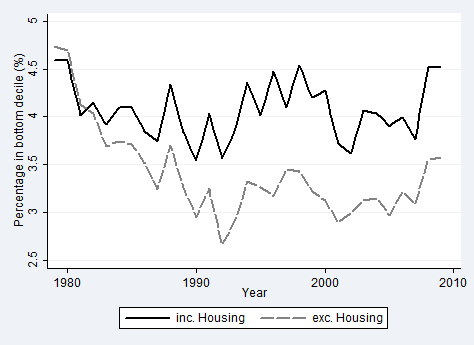
\includegraphics[width=.7\linewidth]{pictures/overlap.png}
\label{fig:overlap}
\end{figure}

[Add notes and sources. Do we need standard errors? Or an y-axis that starts at zero?]

\subsection{The composition of the ``income poor'' and the ``consumption poor''}\label{subsec:composition}
%Given the differences in ranking between resource distributions, there are a number of individuals for whom resource distribution matters for whether they are identified as having low living standards: they would be classed as living in poverty if their living standards were measured using income but not if they were measured by consumption and vice versa. It is informative to dig deeper into differences in the characteristics of the individuals who make up the bottom deciles of the different resource distributions.

%We begin with a simple descriptive analysis.
%We now examine the composition of the bottom of each of the income and consumption distribution. 

%We begin with a relatively simple breakdown, asking to what extent individuals with the lowest resources are the elderly, or are children. 

Figure \ref{fig:age_comp} shows, in each year and for each of our four measures of household resources, the proportion of the bottom decile group who are working-age adults, the elderly (defined as [?XXXX?])or dependent children.\footnote{We produce these figures with an individual-level (rather than household-level) analysis, where each individual in the sample is assigned their household's equivalised income or consumption. The bottom decile group is therefore defined as the poorest 10 \% of individuals with the lowest equivalised household income or consumption.} There is a consistent story across all measures that the proportion of the bottom decile group who are pensioners is considerably lower in 2009 than it was in 1979. But the extent to which the group deemed to have low resources contains the elderly depends on how resources are measured. Two facts are clear. First, regardless of the treatment of resources from housing, the proportion of the bottom decile group who are the elderly is lower when assessed using income than when using consumption.\footnote{Crossley and O'Dea (2010) present an analysis that is consistent with this finding by showing the median saving rate (defined as \emph{income less spending} as a fraction of \emph{income} by age that is implied by the same LCFS data as we analyse here. These implied saving rates rise strongly with age for those aged over 60; equivalently, many elderly households report in the LCFS cash spending levels that are considerably lower than their cash income. This seems counter-intuitive, at least if one has in mind a simple lifecycle model of asset accumulation and decumulation. Finch and Kemp (2006), analysing the same data that we use, concluded that ``although the evidence has been far from conclusive, low spending amongst pensioner households appears to reflect an inter-related set of factors associated with increasing frailty and declining mobility, leading to reducing social participation and contracting social networks.'' Put more crudely, they found no evidence that the data was under-recording spending, and attributed the low levels of spending to a declining ability (or need) to spend money as older people's health deteriorated. Using qualitative research, Dominy and Kempson (2006) found considerable evidence of saving going on amongst the elderly, much of which would probably be considered by economists as precautionary saving for unexpected, lumpy items of spending. In the absence of high-quality longitudinal data on household wealth, more research is needed before we can conclude whether the LCFS is offering a correct impression of the savings behaviour of the elderly, and if so, what economic explanation lies behind it. Until, we need to be mindful that income and consumption do give differing impressions of the living standards of the elderly in ways which may be different from conventionally assumed. We will return to this discussion in Section \ref{sec:housing}.} Second, moving to a measures of resources that includes the imputed resources from housing reduces the proportion of the bottom decile group who are elderly (and particularly so when using consumption). By contrast, working-age adults and children are more likely to be income-poor than consumption-poor; adding the imputed consumption from housing makes working-age adults and children more likely to be consumption-poor; but adding the imputed income from housing makes working-age adults less likely, but children more likely, to be income-poor.

\begin{figure}
\caption{Age Composition of Bottom Decile Group of Income and Consumption}
\centering
	\subfloat[Working age]
	{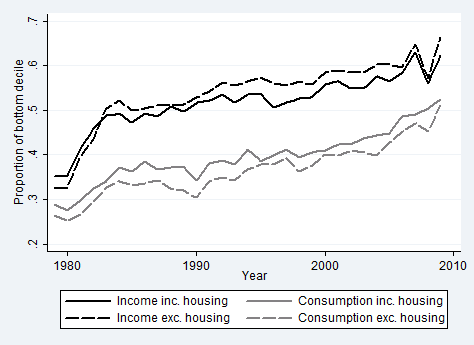
\includegraphics[width=.5\linewidth]{pictures/dec_comp2.png}} \\
	\subfloat[Pensioners]
	{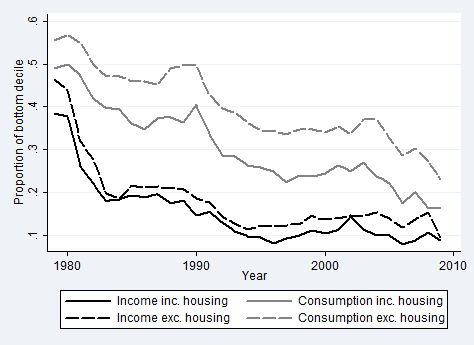
\includegraphics[width=.5\linewidth]{pictures/dec_comp3.png}} \\
	\subfloat[Children]
	{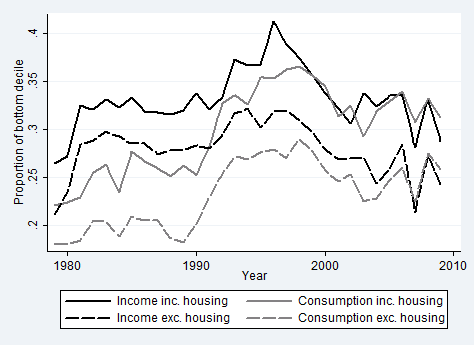
\includegraphics[width=.5\linewidth]{pictures/dec_comp1.png}} \\
\label{fig:age_comp}
\end{figure}

[Need notes and sources. (I think standard errors would clutter this too much).]

Figure \ref{fig:pov_comp} shows the proportion of the bottom decile group with high levels of educational qualifications (defined as leaving school after the age of 16 years old [MIKE ASKS ABI: IS THIS CORRECT? IT's NOT WHAT WE DO LATER ON]). Over time, the bottom decile group (however measured) has become increasingly well educated, in line with population changes over the past forty years. What is more interesting, though, is that those with a low consumption are less likely to be high educated compared to those with a low income. Because we would expect an individual's educational attainment to be strongly correlated with wealth or lifetime resources, then this suggests that taking those with a low consumption as being the poor in society better identifies those more likely to be long-term poor than using income. The same is true, but to a much smaller extent, for moving to a measure of resources that includes the imputed resources from housing, meaning that Figure \ref{fig:pov_comp} also suggests that a measure of resources that includes the imputed resources from housing is (slightly) more likely to identify as poor those in long-term poverty than measures of resources without the imputed resources from housing.

\begin{figure}
\caption{Proportion of More Educated Individuals in Bottom Decile Group of Income and Consumption}
\centering
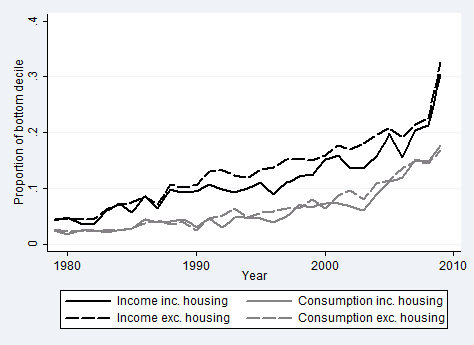
\includegraphics[width=.7\linewidth]{pictures/dec_comp4.png}
\label{fig:pov_comp}
\end{figure}

To probe this suggestion further, and examine multiple characteristics simultaneously, Table \ref{table:multinom_incon} shows relative risk ratios of several demographic characteristics for the outcomes ``in the bottom decile group of both income and consumption resource distributions'', $r_{IC}$, ``in the bottom decile group of the income distribution but not the consumption distribution'', $r_{I}$, and ``in the bottom decile group of the consumption distribution but not the income distribution'', $r_{C}$, with ``not in the bottom decile group of either the income and consumption distributions'' as the reference category. \footnote{The results given here are for the sub-period 1999-2009. The results for earlier decades show the same qualitative story, and can be found in the Appendix \ref{sec:annex_results}.} The key parameter of interest, reported in the column titled $r_{I}-r_{C}$, is then the difference between the relative risk ratio of being ``in the bottom decile group of the income distribution but not the consumption distribution'' and ``in the bottom decile group of the consumption distribution but not the income distribution'', and we report the $\chi^{2}$ test statistic for this difference being zero. \footnote{An alternative approach would be to estimate separate logits for being in the bottom decile group of income and of consumption, and comparing coefficients across models. However, as noted in Allison (1999), coefficients in binary regression are confounded with residual variation, and so differences in the amount of residual variation between groups can produce differences in slope coefficients between groups that are not indicative of causal differences. Although solutions have been proposed to deal with this problem, all have their drawbacks (see, for example, Williams (2009) and Mood (2010)) and there is yet no consensus. We therefore we estimate a multinomial logit model and test for significant differences in the impact that characteristics have in predicting income-only-poverty versus consumption-only-poverty. If a characteristic was just as effective at predicting income-poverty as it was consumption-poverty - which is the interpretation that people like to make when logit coefficients are found to be equal to each other - then these relative risk ratios in our multinomial logit should not be significantly different from each other.} To give an example of how to interpret the table, recall that Figure \ref{fig:pov_comp} showed that the bottom decile group of the consumption distribution contained more low-educated individuals than the bottom decile group of the income distribution, meaning that having a low education is a better predictor of having a low consumption than it is of having a low income. This is reflected in the left-hand panel of Table \ref{table:multinom_incon}, where there is a higher relative risk ratio on ``left school $\leq16$'' in column $r_{C}$ (2.460) than there is in column $r_{I}$ (1.300). The fourth column of the left-hand panel, $r_{I}-r_{C}$, reports the difference in these relative risk ratios, confirming that it is negative, and statistically different from zero at the 5\% level. The interpretation is, therefore, that  having a low education is more strongly correlated with having a low consumption than having a low income. 

%The results are in Table \ref{table:multinom_incon}, which shows the relative risk ratios of several demographic characteristics for the outcomes ``in the bottom decile group of both income and consumption resource distributions'', $r_{IC}$, ``in the bottom decile group of the income distribution but not the consumption distribution'', $r_{I}$, and ``in the bottom decile group of the consumption distribution but not the income distribution'', $r_{C}$. 

Overall, remembering that a negative value in the $r_{I}-r_{C}$ column means that that demographic characteristic is a better predictor of having a low consumption than it is for having a low-income, the left-hand panel of Table \ref{table:multinom_incon} shows that the risk of being in the bottom decile group of the income distribution but not of the consumption distribution is higher for those who are: under 30, highly educated, being self-employed, not being in paid employment (called ``workless'' in the table), and those who live in a single adult or couple household (the right-hand panel of Table \ref{table:multinom_incon} repeats the analysis using measures of income and consumption that do not add the imputed resources from housing, and the conclusions are very similar).\footnote{The finding for the self-employment is fully in line with previous work, and is usually taken to being caused by significant under-reporting of income by the self-employed: Brewer et al. (2009) and Brewer et al. (2016) both show that, conditional on reported household income, self-employed households enjoy a greater standard of living (measured by level of expenditure, or the food share of the total budget) than employed households.} Conversely, the risk of being in the bottom decile group of the consumption distribution but not of the income distribution is higher for those who: are over 60, have a low education, are in work, and live in a household with children. Our interpretation of these results is that those found at the bottom of the income distribution are those who are more likely to be temporarily poor - the young, those with high levels of education, and those out of work (many of whom will soon move into work) - than those found at the bottom of the consumption distribution. [Mike says: although I note that there is an issue with age, and the non-spending older people. REFER BACK TO EARLIER DISCUSSION].  

\begin{sidewaystable}
\caption{Demographics and the Bottom Decile, 1999-2009: Multinomial Logit Relative Risk Ratio [Mike asks Abi and Cormac: can you provide a more informative or descriptive title]}
\centering
\begin{tabular}{l|cccc|cccc}
\hline\hline
	& \multicolumn{4}{c}{\textbf{IHC Bottom Decile}} &  \multicolumn{4}{c}{\textbf{XHC Bottom Decile}} \\
	&	Inc \& Cons.	&	Inc. Only	&	Cons. Only	&	Diff.	&	Inc \& Cons	&	Inc Only	&	Cons. Only	&	Diff. 	\\
	&	$r_{IC}$	&	$r_{I}$	&	$r_{C}$ &	$r_{I}$-$r_{C}$&	$r_{IC}$	&	$r_{I}$	&	$r_{C}$	&	$r_{I}$-$r_{C}$\\
 & se & se & se & $\chi^{2}$  & se & se & se & $\chi^{2}$ \\
\hline
Left school $\leq$ 16	&	       2.370***	&	       1.20***	&	       2.68***	&	-1.48***	&	     					  1.47*** 	&	1.07	&	       2.21***	&	-1.14***	\\
                    	&	       0.252   	&	0.09	&	0.28	&	58	
		&	       0.088   	&	0.06	&	0.15	&	55	\\
Left school $>$ 19	&	       1.71***   	&	       0.92  	&	       0.99* 	&	-0.07	&
				       0.85*   	&	0.94	&	0.96	&	-0.02	\\
                    	&	       0.177   	&	0.07	&	0.11	&	0.25	&	
			      0.069   	&	0.09	&	0.07	&	0.05	\\
Age $<$ 30	&	       1.150   	&	       1.55***	&	1.32***	&	0.23***	&
			       1.21*   	&	       1.36***	&	1.25***	&	0.10	\\
                    	&	       0.142   	&	0.11	&	0.12	&	4.51	&	
			       0.133   	&	0.08	&	0.10	&	1.9	\\
Age 30-40	&	       1.032   	&	1.14**	&	       1.11** 	&	0.03	&	
			       0.85***	&	1.02	&	1.09***	&	-0.07	\\
                    	&	       0.068   	&	0.07	&	0.05	&	0.12	&	
			       0.047   	&	0.05	&	0.05	&	0.64	\\
Age 50-60	&	       0.791**  	&	       0.85*** 	&	0.96	&	-0.11	&
			       0.91   	&	       0.82***  	&	1.02	&	-0.20***	\\
                    	&	       0.093   	&	0.04	&	0.03	&	3.22	&	
			       0.055  	&	0.04	&	0.06	&	7.00	\\
Age 60-70	&	       0.263***	&	       0.41***	&	       1.00 	&	-0.59***	&	       						0.14***	&	       0.36***	&	1.10	&	-0.74***	\\
                    	&	       0.034   	&	0.04	&	0.08	&	46.51	&	
			    0.012   	&	0.03	&	0.07	&	113	\\
Age $\geq$ 70	&	       0.331***	&	       0.20***	&	       2.12***	&	-1.92***	&	       					0.20***	&	       0.21***	&	       2.46***	&	-2.25***	\\
                    	&	       0.051   	&	0.02	&	0.18	&	284	&	       0.03   	&	0.01	&	0.24	&	445	\\
Workless	&	       13.130***	&	       6.57***	&	       3.17***	&	3.41***	&	       						17.2***	&	       7.54***	&	       3.54***	&	4.00***	\\
	&	1.33	&	0.52	&	0.26	&	42	&	
	1.43	&	0.38	&	0.18	& 	82 \\
Self Employed	&	       13.130***	&	       3.88***	&	       0.92 &	2.96***	&	       							1.64***	&	       4.23***	&	       0.89 &	3.34***	\\
	&	1.33	&	0.35	&	0.08	&	88	&
		0.20	&	0.37	&	0.09		& 121	\\
Couple	&	      0.776***	&	       0.85***	&	      0.72***	&	0.13**	&	       						0.96	&	      1.11	&	      0.93	&	0.19**	\\
			&	0.069	&	0.08	&	0.05	&	5.5	&
			0.07	&	0.10	&	0.06		&4.3	\\
Single	&	     0.993	&	       1.14	&	      0.90	&	0.24**	&
		       3.43***	&	       2.22***	&	       2.42***	&	-0.21	\\
	&	0.101	&	0.12	&	0.07	&	6.5	&
		0.280	&	0.19	&	0.17		& 0.9	\\
Children	&	      2.707***	&	       1.53***	&	       2.63***	&	-1.10***	&	       					0.85***	&	       1.12	&	       1.81***	&	-0.69***	\\
	&	0.234	&	0.12	&	0.09	&	124	&	
		0.066	&	0.08	&	0.06		& 55	\\
Constant            	&	       0.013***	&	       0.056***	&	       0.085***	&		&	      					 0.02***	&	       0.069***	&	       0.074***	&		\\
                    	&	       0.00   	&	0.01	&	0.01	&		
		&	       0.00   	&	0.01	&	0.01	&		\\
\hline\hline
\multicolumn{9}{l}{Significantly different from zero at the  10\% ($\star$), 5\% ($\star\star$) and 1\% level ($\star\star\star$).} \\
\multicolumn{9}{l}{Omitted variables: Left school between 17-18 years old; household head aged between 40 and 50 years; employed; multi-family household. }
\end{tabular}
\label{table:multinom_incon}
\end{sidewaystable}


%\subsection{Need title?}

Table \ref{table:interact} explores this conclusion further by interacting employment status with both age and education. As in Table \ref{table:multinom_incon}, the $r_{I}-r_{C}$ column of the left-hand panel of Table \ref{table:interact} shows that having a low education and being aged over 60 are both still stronger predictors of being in consumption-poverty than income-poverty, and that being out of work continues to be more associated with being in income-poverty than consumption-poverty.\footnote{Results in the right-hand panel are qualitatively identical.} What the interactions tells us is that being out of work and having a low education, or being out of work and aged 60 or more, are in fact more strongly associated with consumption-poverty than income-poverty (relative to being out of work and aged under 60, or being out of work with a high level of education. If we think that those who with high levels of education more likely to experience being out of work as a temporary phenomenon that those with low levels of education, and if we think that those who are still of working age are more likely to experience being out of work as a temporary phenomenon than those aged 60 or more, then, as before, having this reinforces the conclusion that having a low consumption seems more likely to identify those individuals who are at greater risk of long-term poverty than having a low income.


\begin{sidewaystable}
\caption{Age, Education \& Unemployment, 2000-2009: Multinomial Logit Relative Risk Ratio}
\centering
\begin{tabular}{l|cccc|cccc}
\hline\hline
	& \multicolumn{4}{c}{\textbf{IHC Bottom Decile}} &  \multicolumn{4}{c}{\textbf{XHC Bottom Decile}} \\
	&	Inc \& Cons.	&	Inc Only	&	Cons. Only	&	Diff.	&	Inc \& Cons	&	Inc Only	&	Cons. Only	&	Diff. 	\\
	&	$r_{IC}$	&	$r_{I}$	&	$r_{C}$ &	$r_{I}$-$r_{C}$&	$r_{IC}$	&	$r_{I}$	&	$r_{C}$	&	$r_{I}$-$r_{C}$\\
 & se & se & se & $\chi^{2}$  & se & se & se & $\chi^{2}$ \\
\hline
Left school $\leq$ 16	&	       2.63***	&	       1.32***	&	       2.25***	&	-0.92***	&	       						1.20   	&	       1.20***  	&	      1.96***	&	-0.75***	\\
                    				&	       0.43   	&	0.09	&	0.21	&	21	&	
			      				 0.18   	&	0.08	&	0.17	&	20	\\
Left school $>$ 19	&	       1.13   	&	       0.71***	&	       0.81*** 	&	-0.10	&	       						0.62**   	&	       0.82** 	&	0.93	&	-0.12	\\
                   	 	&	       0.23   	&	0.06	&	0.10	&	0.80	&	
			  	   0.12   	&	0.06	&	0.10	&	1.00	\\
Workless*Left school $\leq$ 16	&	       0.90   	&	0.86	&	       1.39**  	&	-0.53***	&	       					1.27  	&	       0.82**  	&	1.021	&	-0.39***	\\
                    	&	       0.17   	&	0.09	&	0.19	&	8.7	&
	       0.22   	&	0.08	&	0.14	&	7.4	\\
Workless*Left school $>$ 19	&	       2.10***   	&	       1.96***	&	1.48**	&	0.49	&	       1.63 **  	&	       1.39***	&	1.01	&	0.38***	\\
	&	       0.50   	&	0.25	&	0.28	&	1.7	&
	       0.37   	&	0.17	&	0.16	&	3.0	\\
Age $<$ 30	&	       1.30*  	&	       1.62*** 	&	1.35***	&	0.27	&	
			       1.07   	&	1.25***	&	1.27**	&	-0.02	\\
	&	       0.20   	&	0.15	&	0.14	&	1.8	&	
			    0.19  	&	0.11	&	0.13	&	0.01	\\
Age 30-40	&	       0.85   	&	1.11	&	       1.132 	&	-0.02	&	
			       0.78  	&	      0.97  	&	1.08	&	-0.11	\\
                    	&	       0.11  	&	0.08	&	0.09	&	0.03	&	
			       0.13   	&	0.06	&	0.09	&	1.12	\\
Age 50-60	&	       0.70**  	&	0.84**	&	0.82**	&	0.02	&	
			       0.95   	&	       0.81***  	&	0.99	&	-0.18	\\
                    	&	       0.12  	&	0.07	&	0.08	&	0.04	&	
			       0.16   	&	0.06	&	0.10	&	2.7	\\
Age 60-70	&	       0.47** 	&	0.72***	&	       1.245**	&	-0.52***	
		&	       0.42*** 	&	       0.62***	&	1.28	&	-0.66***	\\
                    	&	       0.14   	&	0.09	&	0.17	&	5.32	&	
			       0.13   	&	0.07	&	0.16	&	20	\\
Age $\geq$ 70	&	       0.34***	&	       0.18***	&	       1.99***	&	-1.81***	&	       						0.21***	&	       0.21***	&	       2.29***	&	-2.08***	\\
                    	&	       0.03   	&	0.02	&	0.17	&	452	&	
			      0.02   	&	0.02	&	0.18	&	573	\\
Workless*Age $<$ 30	&	       0.87   	&	0.82	&	0.84	&	-0.102
				&	       1.23   	&	1.16	&	0.91	&	0.25	\\
				&	       0.16  	&	0.11	&	0.13	&	0.03	&	
					   0.25   	&	0.15	&	0.14	&	2.0	\\
Workless*Age 30-40	&	       1.30*   	&	1.03	&	0.93	&	0.10	&	
				       1.11   	&	1.14	&	0.97	&	0.17	\\
			&	       0.20   	&	0.12	&	0.12	&	0.44	&	
				      0.20   	&	0.12	&	0.12	&	1.3	\\
Workless*Age 50-60	&	       1.15  	&	0.95	&	1.28	&	-0.32	&	
				       0.93   	&	0.97	&	1.01	&	-0.04	\\
			&	       0.22   	&	0.11	&	0.18	&	2.9	&	
				   0.17   	&	0.10	&	0.13	&	0.1	\\
Workless*Age 60	&	       0.52**   	&	       0.47***	&	       0.73**  	&	-0.26**	&	
			   0.31***	&	       0.52***	&	0.77	&	-0.25**	\\
	&	       0.17   	&	0.06	&	0.11	&	4.7	&	
		       0.09   	&	0.07	&	0.11	&	4.6	\\
Workless	&	       11.8***	&	       7.22***	&	       2.48***	&	4.73***	
		&	       13.9***	&	       8.14***	&	       3.30***	&	4.85***	\\
		&	       2.40   	&	0.84	&	0.37	&	35	
		&	       2.61   	&	0.87	&	0.44	&	32	\\
Self emp	&	       1.30*	&	       3.80***	&	      0.91	&	2.89***	
		&	       1.52**	&	       4.09***	&	       0.91 &	3.18***	\\
		&	       0.19   	&	0.22	&	0.09	&	166	
		&	       0.26   	&	0.22	&	0.09	&	184	\\
Couple	&	       0.84**	&	      0.91	&	     0.75**	&	0.16***	
		&	       1.02	&	       1.16**	&	      0.98	&	0.18**	\\
		&	       0.07   	&	0.05	&	0.05	&	5.8	
		&	       0.10   	&	0.07	&	0.06	&	4.3	\\
Single	&	       1.06	&	       1.23*** 	&	   0.93	&	0.30***	
		&	       3.66***	&	     2.32***	&	       2.52***	&	-0.21	\\
		&	       0.08   	&	0.07	&	0.06	&	12	
		&	       0.31   	&	0.13	&	0.16	&	1.1	\\
Children	&	       2.68***	&	     1.52***	&	      2.65***	&	-1.13***	
		&	       0.86***	&	      1.10**	&	       1.83***	&	-0.73***	\\
		&	       0.17   	&	0.07	&	0.15	& 67	
		&	       0.05   	&	0.05	&	0.10	& 64	\\
Constant            	&	       0.01***	&	       0.04***	&	       0.03***	&		&	       0.02***	&	       0.04***	&	       0.03***	&		\\
                    	&	       0.002   	&	0.004	&	0.001 	&		&	       0.003   	&	0.004	&	0.003	&		\\
\hline\hline
\multicolumn{9}{l}{Significantly different from zero at the 10\% ($\star$), 5\% ($\star\star$) and 1\% level ($\star\star\star$).} \\
\multicolumn{9}{l}{Omitted variables: Left school between 17-18 years old; household head aged between 40 and 50 years; employed; multi-family household.}
\end{tabular}
\label{table:interact}
\end{sidewaystable}




NEW TEXT BASED ON NEW TABLES NOT CONTAINED IN THIS DOCUMENT. 25 FEB.  VERSION WITH SINGLE INTERACTED WITH OVER 60: Overall, remembering that a negative value in the $r_{I}-r_{C}$ column means that that demographic characteristic is a better predictor of having a low consumption than it is for having a low-income, the left-hand panel of Table \ref{table:multinom_incon} shows that the risk of being in the bottom decile group of the income distribution but not of the consumption distribution is higher for those who are: self-employed, not in paid employment (called ``workless'' in the table), living in single adult households (and of working age), and home-owners.\footnote{The finding for the self-employment is fully in line with previous work, and is usually taken to being caused by significant under-reporting of income by the self-employed: Brewer et al. (2009) and Brewer et al. (2016) both show that, conditional on reported household income, self-employed households enjoy a greater standard of living (measured by level of expenditure, or the food share of the total budget) than employed households.} In the other direction, the risk of being in the bottom decile group of the consumption distribution but not of the income distribution is higher for those who: are over 60 (and even more so for those who live in single adult households), have a low education, and live in a household with children. (The right-hand panel of Table \ref{table:multinom_incon} repeats the analysis using measures of income and consumption that do not add the imputed resources from housing, and the conclusions are very similar, other than living in a single adult household loses its importance). Our interpretation of these results is that those found at the bottom of the income distribution are those who are more likely to be temporarily poor - home-owners, adults living alone, those with high levels of education, and those out of work (many of whom will soon move into work) - than those found at the bottom of the consumption distribution, who are more likely to have characteristics suggesting that they are permanently poor - low levels of education, and having dependent children. There is also a difference in the age profile, particularly at older ages, with the risk of consumption poverty rising much steeply with age for those aged 70 or over.

NEW TEXT BASED ON NEW TABLES NOT CONTAINED IN THIS DOCUMENT. 25 FEB.  VERSION WITH SINGLE INTERACTED WITH OVER 60 AND WITH EMPLOYMENT STATUS INTERACTED WITH AGE AND EDUCATION: Table XXX explores this conclusion further by interacting employment status with both age and education. As in Table XXX, the $r_{I}-r_{C}$ column of the left-hand panel of Table XXX shows that having a low education, having children, and being aged over 70 (or aged over 60 and living alone) are all still stronger predictors of being in consumption-poverty than income-poverty, and that being out of work or self-employed continues to be more associated with being in income-poverty rather than consumption-poverty.\footnote{As before, results in the right-hand panel are qualitatively identical.} What the interactions tell us is that being out of work and having a low education is more strongly associated with consumption-poverty than income-poverty, but that being out of work and having a high education is more strongly associated (albeit without statistical precision) with income-poverty than consumption-poverty. If we think that those who with high levels of education more likely to experience being out of work as a temporary phenomenon that those with low levels of education, then, this reinforces the conclusion that having a low consumption seems more likely to identify those individuals who are at greater risk of long-term poverty than does having a low income. Similarly, the interaction between age and employment status shows that not being in work more strongly predicts consumption poverty than income poverty amongst those aged 50 or over, for whom not being in work is more likely to be a permanent situation than those who are young and not in paid work. 


\subsection{The standard of living of the ``income poor'' and the ``consumption poor''}\label{subsec:DiDs}

Section \ref{subsec:mismatch} showed that income and consumption give different orderings of households and identify different households as having low resources, and 
Section \ref{subsec:composition} suggested that having a low consumption is more likely to identify those individuals who are at greater risk of long-term poverty than having a low income. In this section, we provide a complementary analysis by showing which of having a low consumption and a low income better correlates with other indicators of having low living standards. 

Following \citet{meyer2003measuring}, we define four groups $BrInc_{low}$. $BrInc_{notlow}$, $Con_{low}$
and $Con_{notlow}$, where the subscript `low' refers to those households
lying in the bottom 10 per cent of the consumption or income distribution,
and `notlow' to those households lying in the upper 90 per cent of
the distribution in question, and BrInc and Con refer to broad income and consumption respectively. If 
$X$ is an outcome that correlates positively
with living standards, and $X(y)$ is defined as the mean outcome for group
$y$, we then calculate:

\begin{equation}
\left[X(Con_{low})-X(Con_{notlow})] - [X(BrInc_{low})-X(BrInc_{notlow})\right]\label{eq:diffindiff}
\end{equation}

This difference-in-difference type measure will be negative if being in the bottom decile group of reported
consumption is a better indicator of poor outcomes (as measured by $X$) than being in the
bottom decile group of reported income.

The results are shown in Table \ref{tab:Rel_cons_inc_all}. We calculate this measure for ownership of various consumer durables
(dishwasher, washing machine, central heating, computer, DVD player,
access to the internet at home, a TV, subscription TV); having private health
insurance; owning one or more cars; owning their own house; and the
number of rooms in the house. \footnote{As noted above, the measure of consumption
used here does not include any spending on durables, meaning that we do not have a mechanical relationship
between the measure of consumption and the outcomes of interest.} All but
one of the statistics have a negative sign and are statistically significant;
the exception is owning a TV, which could reflect that not owning a television is now a sign of preferences, rather than of having low resources. 

Although the LCFS provides
a limited number of alternative measures of living standards, 
the results show emphatically that having a low consumption is
a better guide to having a low living standard than having a low
income.

% Table generated by Excel2LaTeX from sheet 'Table 6'
\begin{sidewaystable}
%\begin{table}[htbp]
\centering
\caption{The relationship between low consumption, low income and other outcomes, all households}
\begin{tabular}{lcccccccc}
\addlinespace
\toprule
& (1)    & (2)    & (3)    & (4)    & (5)    & (6)    & (7)    & N \\
\midrule
& $X(Inc_{low})$ & $X(Inc_{notlow})$ & (1)-(2) & $X(Con_{low})$ & $X(Con_{notlow})$ & (4)-(5) & (6)-(3) &  \\
Wsh. Mch. & 0.92  & 0.96  & -0.04 & 0.84  & 0.96  & -0.12 & -0.083*** & 52,796 \\
Cent. Heat. & 0.92  & 0.94  & -0.03 & 0.89  & 0.95  & -0.06 & -0.030*** & 52,796 \\
Dishwash. & 0.20   & 0.36  & -0.16 & 0.06  & 0.37  & -0.31 & -0.151*** & 52,796 \\
DVD   & 0.59  & 0.61  & -0.03 & 0.42  & 0.63  & -0.22 & -0.189*** & 52,796 \\
TV    & 0.98  & 0.99  & -0.01 & 0.98  & 0.99  & -0.01 & 0.002 & 52,796 \\
Pay TV & 0.30   & 0.39  & -0.09 & 0.18  & 0.40   & -0.22 & -0.134*** & 52,796 \\
PC    & 0.54  & 0.64  & -0.10  & 0.24  & 0.68  & -0.44 & -0.335*** & 52,796 \\
Internet & 0.41  & 0.56  & -0.15 & 0.15  & 0.59  & -0.44 & -0.286*** & 52,796 \\
Car   & 0.53  & 0.78  & -0.25 & 0.24  & 0.82  & -0.57 & -0.321*** & 52,796 \\
Two cars & 0.14  & 0.33  & -0.19 & 0.02  & 0.34  & -0.32 & -0.130*** & 52,796 \\
Own hse. & 0.37  & 0.74  & -0.38 & 0.32  & 0.75  & -0.43 & -0.055*** & 52,796 \\
No. rooms & 4.97  & 5.38  & -0.41 & 4.5   & 5.44  & -0.94 & -0.528*** & 52,796 \\
Health ins. & 0.05  & 0.13  & -0.08 & 0.02  & 0.13  & -0.12 & -0.036*** & 52,796 \\
\bottomrule
\multicolumn{9}{c}{\parbox[b]{18cm}{
{\footnotesize{Source: Authors' calculation using Expenditure and Food Survey/Living Costs and Food Survey 2001/02- 2009. \\*
Notes: Column (7) gives the quantity expressed in equation (3). Negative numbers indicate that consumption is better correlated with the outcome in the left-hand column (e.g. having a washing machine, owning one's own home) than is income. Other columns give the individual components of the quantity in equation (3). *** indicates significant at the 1\% level, ** indicates significant at the 5\% level, * indicates significant at the 10\% level. Confidence intervals are calculated by bootstrapping with 999 replications.}}}}
\end{tabular}%
\label{tab:Rel_cons_inc_all}%
%\end{table}%
\end{sidewaystable}%



%
%\subsection{Summmary}
%
%In summary, we have shown that [...].
